\documentclass[12pt,a4paper]{article}
\usepackage[utf8]{inputenc}
\usepackage[danish]{babel}
\usepackage{graphicx}
\usepackage{amsmath}
\usepackage{enumitem}
\usepackage{hyperref}
\usepackage{amsmath}
\usepackage{amssymb}

\title{Algoritmer og Datastrukturer (NDAA04010U) Ugeopgave 5}
\author{Københavns Universitet}
\date{2025}

\begin{document}

\maketitle

\section{Mindste udspændende træ}

Betragt mindste udspændende træ (eng. minimum spanning tree) problemet på denne graf:

\begin{figure}[h]
    \centering
    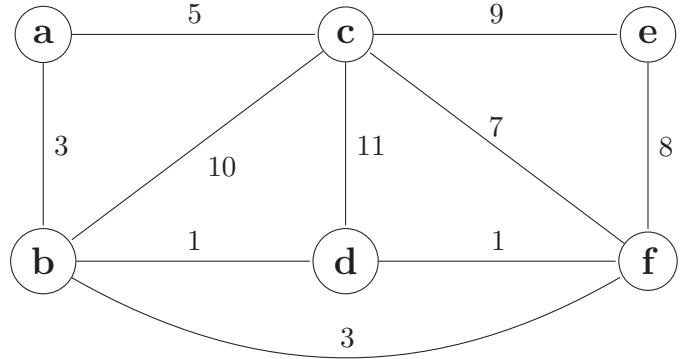
\includegraphics[width=0.7\textwidth]{Ugeopgave_5_markdown/Ugeopgave_5/_page_0_Figure_5.jpeg}
\end{figure}

Hvilke kanter er med i mindste udspændende træ? Angiv for hver kant i træet en snitmængde S hvor kanten er let (eng. light edge) i snittet $(S, V - S)$.

\begin{enumerate}
    \item \{a,b\}
    \item \{a,c\}
    \item \{b,c\}
    \item \{b,d\}
    \item \{b,f\}
    \item \{c,d\}
    \item \{c,e\}
    \item \{c,f\}
    \item \{d,f\}
    \item \{e,f\}
\end{enumerate}

\section{Prim's algoritme}

Betragt følgende vægtede, uorienterede graf:

\begin{figure}[h]
    \centering
    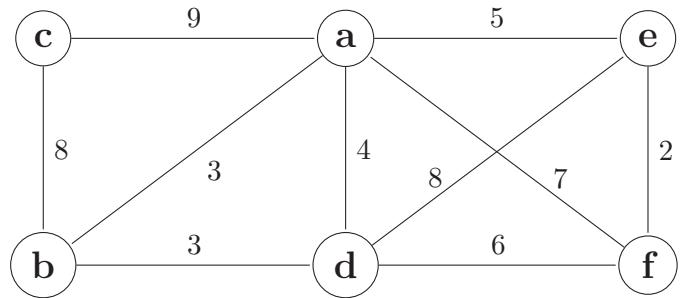
\includegraphics[width=0.7\textwidth]{Ugeopgave_5_markdown/Ugeopgave_5/_page_1_Figure_4.jpeg}
\end{figure}

Hvis Prim's algoritme køres på denne graf med start i knude a, i hvilken rækkefølge bliver knuderne inkluderet i det mindste udspændende træ? (Med andre ord, i hvilken rækkefølge bliver de taget ud af prioritetskøen?)

\begin{enumerate}
    \item a, b, d, e, f, c
    \item a, b, e, d, f, c
    \item a, b, d, c, f, e
    \item a, b, e, f, d, c
\end{enumerate}

\section{Snit og sikre kanter}

Betragt følgende uorienterede, vægtede graf med knudemængde $V = \{a, b, c, d, e, f\}$:

\begin{figure}[h]
    \centering
    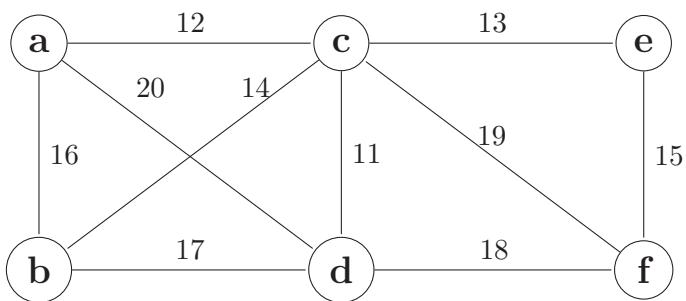
\includegraphics[width=0.7\textwidth]{Ugeopgave_5_markdown/Ugeopgave_5/_page_1_Figure_12.jpeg}
\end{figure}

Betragt kantmængden $A = \{\{a, c\}, \{c, d\}\}$, som er en delmængde af et minimalt udspændende træ (eng. minimum spanning tree). Vi er interesserede i snit (eng. cuts), sikre kanter (eng. safe edges) for A, og snit der respekterer (eng. respects) en kantmængde A. Hvilke af følgende udsagn er sande?

\begin{enumerate}
    \item Lad $S_1 = \{a, b, c, d\}$. Snittet $(S_1, V - S_1)$ respekterer kantmængden A.
    \item Lad $S_2 = \{a, c, e\}$. Snittet $(S_2, V - S_2)$ respekterer kantmængden A.
    \item Lad $S_3 = \{b, e, f\}$. Snittet $(S_3, V - S_3)$ respekterer kantmængden A.
    \item $\{d, f\}$ er en sikker kant for A.
    \item $\{c, e\}$ er en sikker kant for A.
    \item $\{a, d\}$ er en sikker kant for A.
\end{enumerate}

\section{Korteste veje}

Betragt korteste veje problemet (eng. single-source shortest-paths problem) med startknude a på følgende graf:

\begin{figure}[h]
    \centering
    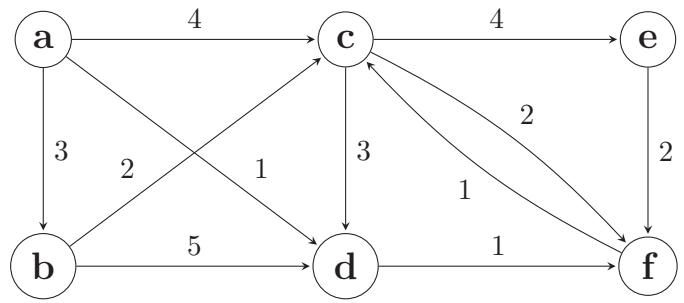
\includegraphics[width=0.7\textwidth]{Ugeopgave_5_markdown/Ugeopgave_5/_page_2_Figure_9.jpeg}
\end{figure}

Hvilke kanter er med i korteste-vej træet? Hvilken algoritme er velegnet til at beregne korteste-vej træet?

\begin{enumerate}
    \item (a,b)
    \item (a,c)
    \item (a,d)
    \item (b,c)
    \item (b,d)
    \item (c,d)
    \item (c,e)
    \item (c,f)
    \item (d,f)
    \item (e,f)
    \item (f,c)
\end{enumerate}

\section{Korteste veje (fortsat)}

Betragt korteste veje problemet (eng. single-source shortest-paths problem) med startknude a på følgende graf:

\begin{figure}[h]
    \centering
    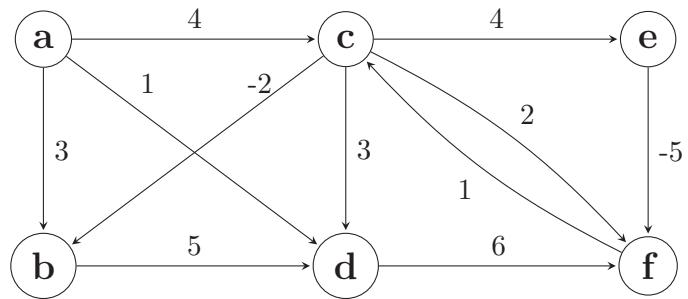
\includegraphics[width=0.7\textwidth]{Ugeopgave_5_markdown/Ugeopgave_5/_page_3_Figure_7.jpeg}
\end{figure}

Hvilke kanter er med i korteste-vej træet? Hvilken algoritme er velegnet til at beregne korteste-vej træet?

\begin{enumerate}
    \item (a,b)
    \item (a,c)
    \item (a,d)
    \item (b,d)
    \item (c,b)
    \item (c,d)
    \item (c,e)
    \item (c,f)
    \item (d,f)
    \item (e,f)
    \item (f,c)
\end{enumerate}

\section{Korteste-veje træ}

Betragt et korteste veje problem på en orienteret graf $G = (V, E)$ (eng. single-source shortest-paths problem on a directed graph) med vægtfunktion $w : E \to \mathbb{R}$ og startknude s. Hvilke af følgende egenskaber har et korteste-veje træ (eng. shortest-paths tree) $G' = (V', E')$ altid?

\begin{enumerate}
    \item I $G'$ kan alle knuder i V nås fra s.
    \item Knuden s har kun udgående kanter i $G'$.
    \item $G'$ har $|V'| - 1$ kanter.
    \item Hvis alle vægte er unikke indeholder $G'$ af de $|E'|$ kanter i G, der har lavest vægt.
    \item $G'$ indeholder den kant i G, der har lavest vægt.
    \item Enhver sti i $G'$ er en korteste vej i G.
    \item Alle korteste veje i G svarer til en sti i $G'$.
    \item $G'$ er et binært træ med s som rod.
    \item $G'$ er et mindste udspændende træ (eng. minimum spanning tree).
    \item Kan beregnes med Dijkstra's algoritme.
\end{enumerate}

\section{Valg af datastruktur}

Antag at vi gerne vil skabe en datastruktur Ventetid, der indeholder en mængde af n afgangstidspunkter (ugedag og klokkeslet, fx for en bus). For enkelheds skyld skal der blot holdes styr på én rute og ét stoppested, så den eneste information er afgangstidspunkter. Datastrukturen skal understøtte to operationer: Insert(x), der indsætter et nyt afgangstidspunkt, og HvorLænge(x) der returnerer antal minutter fra tidspunkt x til den næste afgang.

Hvad er det mest passende valg af datastruktur til løsning af dette problem blandt nedenstående, og hvilken worst-case (amortiseret) køretid for HvorLænge(x) bliver resultatet af dette valg? Udtryk svaret som funktion af n.

\begin{enumerate}
    \item Fibonacci hob (eng. Fibonacci heap), tid $O(\lg n)$.
    \item Fibonacci hob (eng. Fibonacci heap), tid $O(1)$.
    \item Rød-sort binært søgetræ (eng. red-black binary search tree), tid $O(1)$.
    \item Rød-sort binært søgetræ (eng. red-black binary search tree), tid $O(\lg n)$.
    \item En dynamisk tabel, tid $O(1)$.
    \item En dynamisk tabel, tid $O(\lg n)$.
\end{enumerate}

\end{document}
